\atspt
\begin{frame}{\ft{Document Viewers Augmented With APIs}}
\section{Publishing Slide 3}
\doubleFrame{Another strategy for interactive publications is linking documents with APIs maintained by publishers, or 
by cultural or educational institutions.}

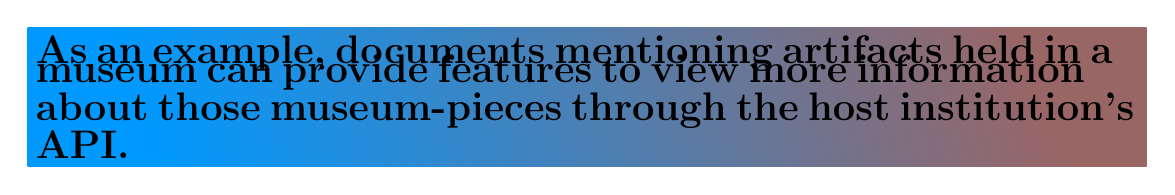
\begin{tikzpicture}
\nodeincludegraphicsTR{2.7cm}{2cm}{pics/Pub-3.png}

 \node [anchor=west,top color=brown!80!blue,
 bottom color=blue!40!cyan, shading angle=290, ,inner sep=3, text width=14cm]
  (longnote) at (2.9,10.3) {\vspace{-7pt}%  %{\color{rb!85!red}{
  {\cframedbox{\Large \textbf{As an example, documents 
mentioning artifacts held in a \makebox{museum} can provide features to 
view more information about those museum-pieces through the host 
institution's API. 
}}}};

\end{tikzpicture}


\end{frame}

